\documentclass{article}

\usepackage{fancyhdr}
\usepackage{lastpage}
\usepackage{extramarks}
\usepackage[usenames,dvipsnames]{color}
\usepackage{courier}
\usepackage{amsmath}
\usepackage{amsthm}
\usepackage{amsfonts}
\usepackage{tikz}

\usetikzlibrary{automata,positioning}

\topmargin=-0.45in
\evensidemargin=0in
\oddsidemargin=0in
\textwidth=6.5in
\textheight=9.0in
\headsep=0.25in

\linespread{1.1}

\pagestyle{fancy}
\lhead{\hmwkAuthorName}
\chead{\hmwkClass\ (\hmwkClassInstructor\ \hmwkClassTime): \hmwkTitle}
\rhead{\firstxmark}
\lfoot{\lastxmark}
\cfoot{}
\renewcommand\headrulewidth{0.4pt}
\renewcommand\footrulewidth{0.4pt}

\setlength\parindent{0pt}

\newcommand{\enterProblemHeader}[1]{
    \nobreak\extramarks{#1}{#1 continued on next page\ldots}\nobreak
    \nobreak\extramarks{#1 (continued)}{#1 continued on next page\ldots}\nobreak
}

\newcommand{\exitProblemHeader}[1]{
    \nobreak\extramarks{#1 (continued)}{#1 continued on next page\ldots}\nobreak
    \nobreak\extramarks{#1}{}\nobreak
}

\setcounter{secnumdepth}{0}
\newcounter{homeworkProblemCounter}

\newcommand{\homeworkProblemName}{}
\newenvironment{homeworkProblem}[1][Problem \arabic{homeworkProblemCounter}]{
    \stepcounter{homeworkProblemCounter}
    \renewcommand{\homeworkProblemName}{#1}
    \section{\homeworkProblemName}
    \enterProblemHeader{\homeworkProblemName}
}{
    \exitProblemHeader{\homeworkProblemName}
}

\newcommand{\problemAnswer}[1]{
    \noindent\framebox[\columnwidth][c]{\begin{minipage}{0.98\columnwidth}#1\end{minipage}}
}

\newcommand{\homeworkSectionName}{}
\newenvironment{homeworkSection}[1]{
    \renewcommand{\homeworkSectionName}{#1}
    \subsection{\homeworkSectionName}
    \enterProblemHeader{\homeworkProblemName\ [\homeworkSectionName]}
}{
    \enterProblemHeader{\homeworkProblemName}
}

\newcommand{\hmwkTitle}{Homework\ \#3}
\newcommand{\hmwkDueDate}{February 14, 2013 at 11:59pm}
\newcommand{\hmwkClass}{CS331}
\newcommand{\hmwkClassTime}{9:00am}
\newcommand{\hmwkClassInstructor}{Professor Zhang}
\newcommand{\hmwkAuthorName}{Josh Davis}

\title{
    \vspace{2in}
    \textmd{\textbf{\hmwkClass:\ \hmwkTitle}}\\
    \normalsize\vspace{0.1in}\small{Due\ on\ \hmwkDueDate}\\
    \vspace{0.1in}\large{\textit{\hmwkClassInstructor\ \hmwkClassTime}}
    \vspace{3in}
}

\author{\textbf{\hmwkAuthorName}}
\date{}

\begin{document}

\maketitle

\pagebreak

\begin{homeworkProblem}
    Prove that if \(L\) is regular, then so is \(L_{\frac{1}{2}}\).
    
    \begin{proof}
        We will show that if \(L\) is regular, then so is \(L_{\frac{1}{2}}\).
        \\
    
        Suppose that \(L\) is regular. Since \(L\) is regular, that means we
        can create a automata for it. Let this automata be \(A\) such that
        \(L(A) = L\). Also let B be an automata such that \(L(B) = L^R\). The
        automata can also be defined as follows:
        \[
            \begin{split}
                A = (Q_A, \Sigma, \delta_A, q_{A}, F_A)
                \\
                B = (Q_B, \Sigma, \delta_B, q_{B}, F_B)
            \end{split}
        \]
        
        
        Since \(L\) is regular, we know that \(L^R\) is also regular because of
        homework two from last week.
        \\

        Now we will make an automata \(C\) constructed from \(A\) and \(B\).
        This will show that \(L_{\frac{1}{2}}\) is regular. \(C\) will be
        defined as follows:

        \[
            C = (Q, \Sigma, \delta, q, F)
        \]

        where

        \begin{enumerate}
            \item \(Q = Q_A \times Q_B\) 
            \item The alphabet is the same, \(\Sigma = \Sigma\)
            \item The start is in the start state for \(A\) and the ending
            state of \(B\), \(q = (q_A, F_B)\).
            \item The final is when we are at the end of \(A\) but the start of
            \(B\), \(F = (F_A, q_B)\)
            \item Define \(\delta\) so that
            \[
                \delta((q_1, q_2), a) = (\delta_A(a), \delta_B(a))
            \]
        \end{enumerate}

        The reason this works is because we just create an automata that is the
        cross product of both of their states. Therefore we create a grid of states. Then
        if we just start at the beginning of \(A\) and the end of \(B\) then only
        accept it when we reach the end of both strings, then it is a valid automata.

    \end{proof}

\end{homeworkProblem}

\pagebreak

\begin{homeworkProblem}
    Let \(w = \sigma_1 \cdots \sigma_n\) be a word on an alphabet \(\Sigma\). By \(w^R\)
    we mean the word is the reverse of w.
    \\
    Define \(L^R\) such that
    \[
        L^R = \{ w \in \Sigma^* : w^R \in L \}.
    \]
    \begin{proof}
        We will show that if \(L\) is regular, then so is \(L^R\).
        \\

        Suppose \(L\) is regular. Since \(L\) is regular, that means we can
        create a NFA for it. Let this NFA, A, be like so:

        \begin{figure}[here]
            \centering
            \begin{tikzpicture}[shorten >=1pt,node distance=2cm,on grid,auto] 
                \node[state, initial] (q_1) [right=of q_0] {$q_1$}; 
                \node[state] (q_2) [right=of q_1] {$q_2$}; 
                \node[state] (q_dots) [right=of q_2] {$\cdots$}; 
                \node[state] (q_{n-1}) [right=of q_dots] {$q_{n-1}$}; 
                \node[state, accepting] (q_n) [right=of q_{n-1}] {$q_n$}; 
                \path[->] 
                    (q_1)
                        edge node {$\sigma_1$} (q_2)
                    (q_2)
                        edge node {$\sigma_2$} (q_dots)
                    (q_dots)
                        edge node {$\sigma_{n-1}$} (q_{n-1})
                    (q_{n-1})
                        edge node {$\sigma_n$} (q_n);
            \end{tikzpicture}
            \caption{NFA, \(A\)}
            \label{fig:automataA}
        \end{figure}

        Now taking this NFA, we can keep the same alphabet \(\Sigma\), states \(Q\),
        but just reverse it to arrive at this NFA, B:

        \begin{figure}[here]
            \centering
            \begin{tikzpicture}[shorten >=1pt,node distance=2cm,on grid,auto] 
                \node[state, accepting] (q_1) [right=of q_0] {$q_1$}; 
                \node[state] (q_2) [right=of q_1] {$q_2$}; 
                \node[state] (q_dots) [right=of q_2] {$\cdots$}; 
                \node[state] (q_{n-1}) [right=of q_dots] {$q_{n-1}$}; 
                \node[state, initial right] (q_n) [right=of q_{n-1}] {$q_n$}; 
                \path[->] 
                    (q_2)
                        edge node {$\sigma_1$} (q_1)
                    (q_dots)
                        edge node {$\sigma_2$} (q_2)
                    (q_{n-1})
                        edge node {$\sigma_{n-1}$} (q_dots)
                    (q_n)
                        edge node {$\sigma_n$} (q_{n-1});
            \end{tikzpicture}
            \caption{NFA, \(B\)}
            \label{fig:automataB}
        \end{figure}

        Since this is a valid NFA, it is exactly the same as Automata \(A\) except
        it has its edges reversed. It only accepts words such that \(w \in L\) and \(w\)
        is reversed.
        \\

        Therefore if \(L\) is regular (it can be represented by a NFA) then
        \(L^R\) is also regular.
    \end{proof}
\end{homeworkProblem}

\begin{homeworkProblem}
    Let \(\Sigma = \{0, 1\}\). Construct a DFA that recognizes the following:
    \[
        \{w \in \Sigma^* : {\left| w \right|}_{01} = {\left| w \right|}_{10}\}.
    \]

    \begin{figure}[here]
        \centering
        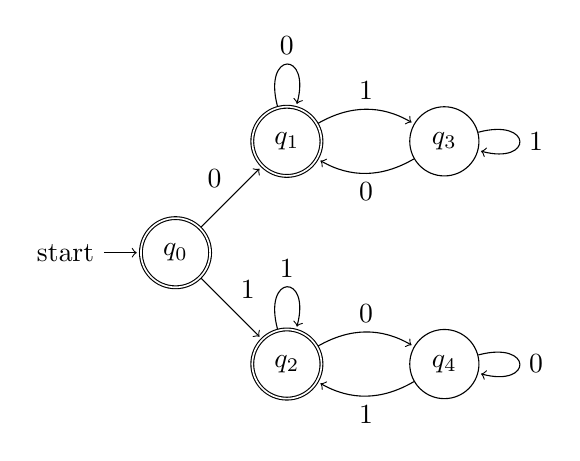
\begin{tikzpicture}[shorten >=1pt,node distance=2cm,on grid,auto] 
            \node[state, initial, accepting] (q_0) {$q_0$}; 
            \node[state, accepting] (q_1) [above right=of q_0] {$q_1$}; 
            \node[state, accepting] (q_2) [below right=of q_0] {$q_2$}; 
            \node[state] (q_3) [right=of q_1] {$q_3$}; 
            \node[state] (q_4) [right=of q_2] {$q_4$}; 
            \path[->] 
                (q_0)
                    edge node {0} (q_1)
                    edge node {1} (q_2)
                (q_1)
                    edge [loop above] node {0} ()
                    edge [bend right=-30] node {1} (q_3)
                (q_2)
                    edge [loop above] node {1} ()
                    edge [bend right=-30] node {0} (q_4)
                (q_3)
                    edge [loop right] node {1} ()
                    edge [bend left] node {0} (q_1)
                (q_4)
                    edge [loop right] node {0} ()
                    edge [bend left] node {1} (q_2);
        \end{tikzpicture}
        \caption{NFA, \(B\)}
        \label{fig:automataB}
    \end{figure}

    This DFA can be shown to be true by using the pumping lemma.

\end{homeworkProblem}

\begin{homeworkProblem}
    Prove that the class of regular languages is closed under imperfect shuffle.

    \begin{proof}
        Consider two regular languages, \(L_A\) and \(L_B\). To show that these
        two languages are closed under the imperfect shuffle, we will construct
        a NFA that can handle these two languages because doing so with a DFA is
        too complicated (similar to how the book uses an NFA to show closure
        under union and concatenation).
        \\

        \textbf{Note:} One thing to note is that this can be shown using a proof
        by induction but NFAs are more fun ;)
        \\

        Consider the two NFAs, \(N_A\) and \(N_B\) such that:
        \[
            \begin{split}
                N_A = (Q_A, \Sigma, \delta_A, q_{A}, F_A)
                \\
                N_B = (Q_B, \Sigma, \delta_B, q_{B}, F_B)
            \end{split}
        \]

        \(N_A\) and \(N_B\) describe two regular languages,
        \(L_A\) and \(L_B\) respectively.
        \\

        The new automata that will show that the two languages are closed
        under the imperfect shuffle can be defined as follows:
        \[
            N = (Q, \Sigma, \delta, q, F)
        \]
        where
        \begin{enumerate}
            \item Two extra states to differentiate
                between which input to expect next \(Q = Q_1 \times Q_2 \times \{A, B\}\) 
            \item The alphabet is the same, \(\Sigma = \Sigma\)
            \item The start is in the start state for \(N_A\) and \(N_B\) and we
            expect an input from \(A\), \(q = (q_A, q_B, A)\).
            \item The final states include both sets and ends with input last from
            \(B\), \(F = F_A \times F_B
            \times \{A\}\)
            \item Define \(\delta\) so that
            \[
                \delta((q_1, q_2, S), a) = \left\{
                    \begin{array}{ll}
                        Q_1 \times Q_2 \times \{B\} \to \mathcal P \left({Q}\right) & \quad S = A \\
                        Q_1 \times Q_2 \times \{A\} \to \mathcal P \left({Q}\right) & \quad S = B
                    \end{array}
                \right.
            \]
        \end{enumerate}
    \end{proof}
\end{homeworkProblem}

\pagebreak

\begin{homeworkProblem}
    Co-determinism.

    \begin{proof}
        \textbf{Show that every CDFA is a DFA.}
        \\

        To do this, we will look at what the differences are between a DFA and
        NFA. A NFA has the following differences:
        \begin{enumerate}
            \item Alphabet = \(\Sigma_{\epsilon}\), allows epsilon transitions
            \item Can have 0 or more transitions for any given input and state
        \end{enumerate}

        A CDFA has already been defined for us. Therefore it has these
        differences from a NFA:
        \begin{enumerate}
            \item Allows only input from \(\Sigma\), no epsilon
            \item Cannot have multiple transitions with the same input going
            into the same state, or \(\delta(q, a) \cap \delta(q', a) =
            \emptyset\)
        \end{enumerate}

        It can be seen that a CDFA and NFA do not share the same properties.
        Therefore a CDFA is just a more specific DFA.
    \end{proof}

    \textbf{Show that every DFA is a CDFA.}
    \\

    \textbf{Counterexample} To show that this is not true, we can take the given
    DFA:
    \begin{figure}[here]
        \centering
        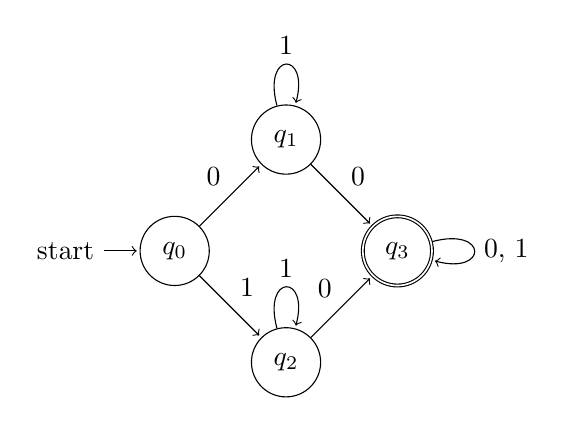
\begin{tikzpicture}[shorten >=1pt,node distance=2cm,on grid,auto] 
            \node[state, initial] (q_0) {$q_0$}; 
            \node[state] (q_1) [above right=of q_0] {$q_1$}; 
            \node[state] (q_2) [below right=of q_0] {$q_2$}; 
            \node[state, accepting] (q_3) [above right=of q_2] {$q_3$}; 
            \path[->] 
                (q_0)
                    edge node {0} (q_1)
                    edge node {1} (q_2)
                (q_1)
                    edge [loop above] node {1} ()
                    edge node {0} (q_3)
                (q_2)
                    edge [loop above] node {1} ()
                    edge node {0} (q_3)
                (q_3)
                    edge [loop right] node {0, 1} ();
        \end{tikzpicture}
        \caption{NFA, \(B\)}
        \label{fig:counterexample1}
    \end{figure}

    The Figure~\ref{fig:counterexample1} is a counterexample because it has
    a state, \(q_3\), that has two incoming arrows for state 0. Thus it violates
    the definition of co-determinism.

    \begin{proof}
        \textbf{Show that every NFA can be converted into an equivalent CDFA.}
        \\\\
        Using the theorem 1.39 out of Sipser's book, it is proven that every NFA
        can be converted into an equivalent DFA.
        \\

        Taking that same DFA, one could add more states to (maximizing) it and
        it would be possible to reduce all same input transisitions to a single
        state down to none such that
        \(\delta(q, a) \cap \delta(q', a) = \emptyset\).
        \\

        Once this has been achieved, the state machine would then be
        co-deterministic.
    \end{proof}
\end{homeworkProblem}

\end{document}
